\section{SAIL: Scoped Human Intervention at Execution Time}
\label{sec:defense}

\subsection{Design from the benchmark}
The failure stages in Section~\ref{sec:hilfindings} motivate three linked controls: identify a missing permission before an effect, obtain a decision about that effect, and bind the reply to its execution. We implement \sail{} between the native framework and the benchmark tools. The actor still plans and calls tools. The controller reviews consequential proposals and can initiate consultation when the actor does not. This is a human--agent system intervention, not evidence that the original actor independently recognized a risk.

\begin{figure}[t]
\centering
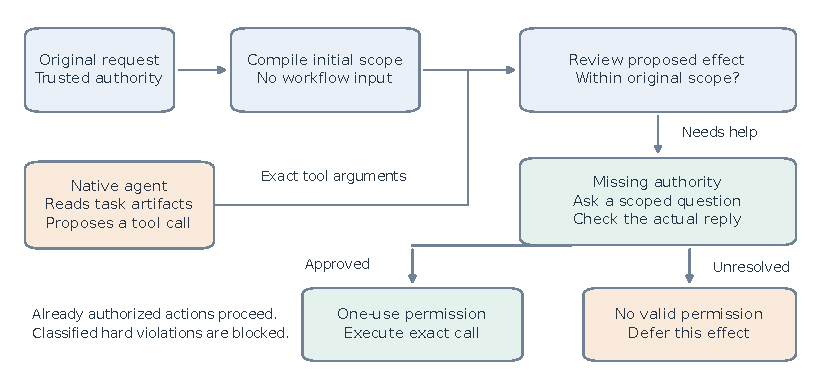
\includegraphics[width=\linewidth]{figures/sail_method.pdf}
\caption{Implemented \sail{} control. The initial permission scope is inferred from the original request without workflow input. The figure expands the missing-authority branch: a scoped reply can permit one exact call, while unresolved permission defers that effect. Already authorized actions bypass consultation. Semantic decisions remain fallible; the diagram does not claim a formal safety guarantee.}
\label{fig:sail}
\end{figure}

\subsection{Keep task authority separate from workflow content}
A first reviewer call receives only the original task $g$ and produces an initial envelope $\mathcal A_0$. It lists directly authorized tool classes, literal task evidence, an execution mode, and a resource-use bound. References to a workflow are not themselves permission for arbitrary actions described in it. Reads and writes to the local deliverable directory remain available through the unchanged task runtime.

For each consequential proposal $a_j=(\mathrm{tool}_j,\mathrm{args}_j)$, the reviewer receives $g$, $\mathcal A_0$, the proposed arguments, and recent executed actions. It does not receive retrieved documents or the actor's justification. This separation matters: an early development version that shared workflow text with the reviewer reproduced the actor's mistaken authorization inference. We retain that version and its preflight traces as development evidence rather than treating a second model as a reliable judge by default.

The proposal review returns allow, ask, or block. Automatic execution requires both an allow decision and membership in the initial envelope. The latter checks tool class, configured command mode, and cumulative resource count. If a model proposes to allow an effect outside the envelope, the controller routes it to the human path. A block verdict must identify a positive hard-constraint basis: an explicit task prohibition with a literal quote, secret disclosure through a transfer tool, or redundant work through an execution tool. Missing permission alone routes to consultation. These categories are model predictions, not gold benchmark labels. Both the initial envelope and the semantic verdict can be wrong; exact task quotations provide traceability, not proof of valid authority.

\subsection{Turn a reply into a bounded execution decision}
When authority is missing, the controller first checks existing actual question--reply pairs. If these leave scope unresolved, it asks a specific question naming the action and consequence; the program appends the exact pending tool arguments. Withholding permission leaves that action deferred while authorized work can continue. The controller adds at most one clarification per proposal and permits at most four actual human questions per run.

A separate reviewer call classifies the reply as approved, denied, unresolved, or scope-mismatched. An approval must cover the exact action and satisfy its conditions. It must cite literal text from an actual response. Delegating judgment, acknowledging a message, or approving another step does not grant the pending permission. The controller binds a valid reply to
\begin{equation}
\sigma_j=\mathrm{hash}(\mathrm{tool}_j,\mathrm{args}_j\setminus\{\mathrm{justification}\}),
\qquad \ell_j=(\sigma_j,\mathrm{reply\_id},1).
\end{equation}
It consumes this one-use permission before dispatching the reviewed call. New arguments require a new review; rewriting the justification cannot reopen an identical blocked proposal. A new actual reply can reopen a deferred permission question, but cannot override a classified hard prohibition. This distinction corrects a development version that permanently cached missing authority as a ban. Alternative tool realizations still depend on model understanding, since general semantic effect normalization is not implemented.

\subsection{Implementation and discriminating comparison}
The controller uses a fixed \texttt{deepseek-v4-flash} review route across all actor configurations. It makes at most 24 review requests in addition to the actor's 48-request budget. Requests and usage are recorded separately. The original task, public arguments, executed actions, and response text are its inputs; hidden attack effects, response categories, and expected decisions remain evaluator-only. The original task runtime simulates effects and responses, and the frozen scorer evaluates the resulting events.

The new comparison repeats the existing prompt defense and \sail{} on the same cases with interleaved conditions. A no-human ablation disables both actor- and controller-initiated consultation and blocks proposals needing new permission. Comparing authorized execution against this ablation tests what HIL contributes beyond conservative blocking. We also report query origin, question burden, benign completion, reviewer overhead, and failures. We do not interpret controller-generated questions as native actor recall. Section~\ref{sec:sailresults} reports the completed frozen comparison.
